\subsection{7 thứ nguyên}
\begin{frame}{7 Đại lượng SI và 7 thứ nguyên}
    \begin{table}
        \centering
        \begin{tabular}{|l|c|c|}
            \hline
            Đại lượng & Ký hiệu & Đơn vị \\
            \hline
            Chiều dài & \(L\) & Meter (m) \\
            \hline
            Khối lượng & \(M\) & Kilogram (kg) \\
            \hline
            Thời gian & \(T\) & Second (s) \\
            \hline
            Cường độ dòng điện & \(I\) & Ampere (A) \\
            \hline
            Nhiệt độ & \(\Theta\) & Kelvin (K) \\
            \hline
            Lượng chất & \(N\) & Mol (mol) \\
            \hline
            Cường độ sáng & \(J\) & Candela (cd) \\
            \hline
        \end{tabular}
        \caption{7 đại lượng cơ bản trong hệ SI và ký hiệu thứ nguyên tương ứng.}
    \end{table}
\end{frame}

\subsection{Phương pháp Rayleigh}
\begin{frame}{Phương pháp Rayleigh}
\vspace{-4mm}
\begin{columns}
\column{0.6\textwidth}

    \begin{itemize}
        \item \(\Delta t^\alpha m^\beta R^\gamma g^\delta \) là đại lượng không thứ nguyên.
    \end{itemize}
    \begin{equation}
        \left[ \Delta t^\alpha m^\beta R^\gamma g^\delta \right] = T^\alpha (M)^\beta (L)^{\gamma + \delta} (T^{-2})^\delta.
    \end{equation}
    nên
    \begin{equation}
        \left\{ \begin{array}{l}
            \alpha - 2\delta = 0 \\
            \beta = 0 \\
            \gamma + \delta = 0
        \end{array} \right.
        \rightarrowtail \left\{ \begin{array}{l}
            \alpha = 2\delta \\
            \beta = 0 \\
            \gamma = -\delta
        \end{array} \right.
    \end{equation}
    Chọn \(\delta = 1\) ta có
    \begin{equation}
        \Delta t = \sqrt{\frac{R}{g}} \ f(\theta).
    \end{equation}

\column{0.4\textwidth}
    \begin{figure}
        \centering
        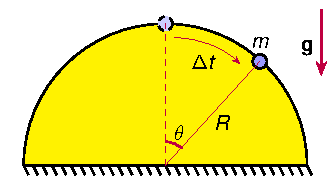
\includegraphics[width=0.9\textwidth]{Figures/Circle_sliding.pdf}
        \caption{Chất điểm trượt trên mặt tròn.}
    \end{figure}
\end{columns}

\end{frame}

\begin{frame}{Khi số biến lớn hơn số bậc tự do?}
\begin{columns}
\column{0.62\textwidth}
    \textbf{Bài toán dao động con lắc lò xo \cite{Lemons_2017}}
    \begin{equation}
        \left[ \omega m^\alpha k^\beta \rho^\gamma V^\delta g^\varepsilon \right]
        = T^{-1 - 2 \beta - 2 \varepsilon} M^{\alpha + \beta + \gamma} L^{3 \delta - 3 \gamma - \varepsilon}.
    \end{equation}
    Giải hệ phương trình và biểu diễn theo 2 biến tự do \(\delta, \varepsilon\):
    \begin{equation}
        \omega m^\alpha k^\beta \rho^\gamma V^\delta g^\varepsilon = \left( \frac{\omega m^{1/2}}{k^{1/2}} \right) \left( \frac{\rho V}{m} \right)^\delta \left( \frac{m^{4/3} g}{k \rho^{1/3}}\right)^\varepsilon.
    \end{equation}
    nên
    \begin{equation}
        \omega = \sqrt{\frac{k}{m}} \ f\left( \frac{\rho V}{m}, \frac{m^{4/3} g}{k \rho^{1/3}} \right).
    \end{equation}

\column{0.38\textwidth}
    \vspace{-8mm}
    \begin{figure}
        \centering
        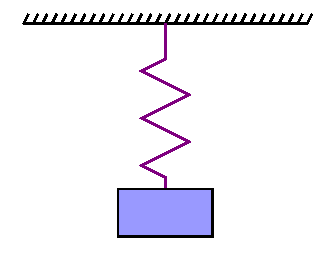
\includegraphics[width=0.9\textwidth]{Figures/Pendulum.pdf}
        \caption{Con lắc lò xo.}
    \end{figure}
    \vspace{-5mm}
    \begin{itemize}
        \item Khối lượng \(m\), độ cứng lò xo \(k\), khối lượng riêng của khí \(\rho\), thể tích chất lỏng \(V\), gia tốc trọng trường \(g\).
        \item Tần số \(\omega = f(m, k, \rho, V, g)\).
    \end{itemize}
\end{columns}
\end{frame}



